\chapter{METHODOLOGY}

\section{System Design}

\begin{figure}[H]
  \centering
  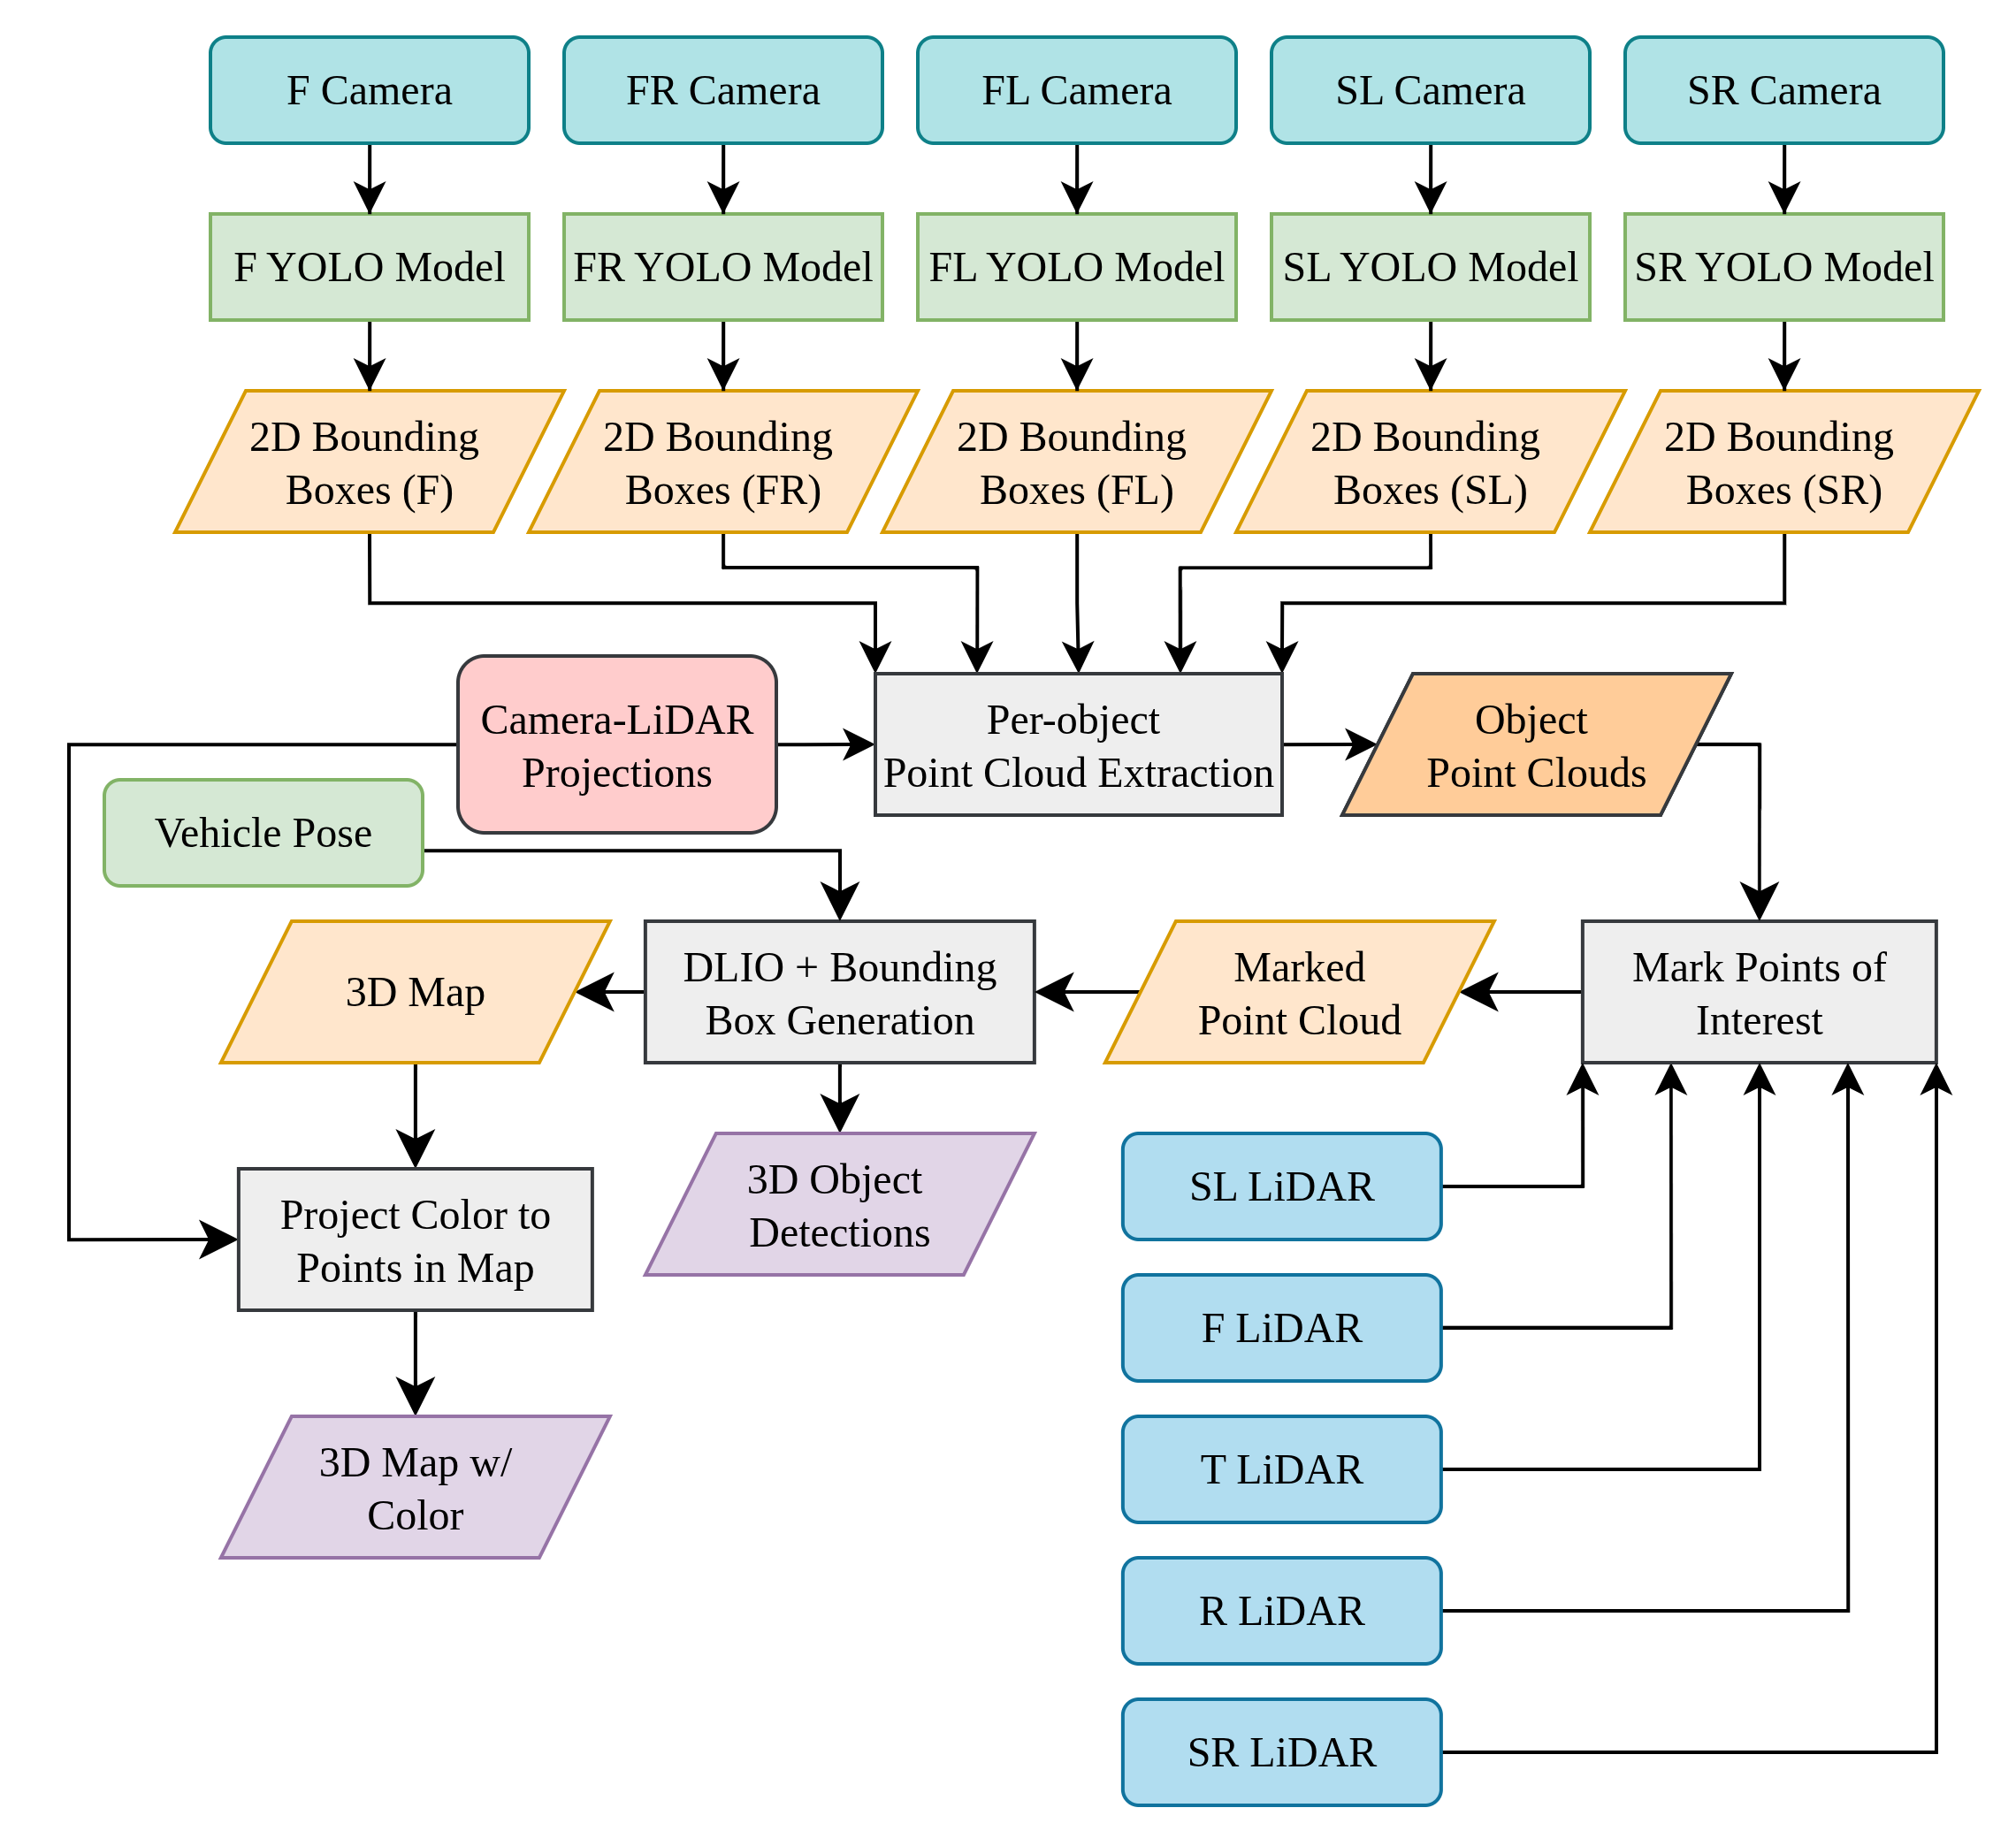
\includegraphics[scale=0.15]{gambar/rt_livo2dm_full.png}
  \caption{Proposed architecture for RT-LIVO2DM}
  \label{fig:rt_livo2dm_full}
\end{figure}

Figure~\ref{fig:rt_livo2dm_full} shows the proposed architecture of the RT-LIVO2DM system. RT-LIVO2DM combines 2D detection results from each camera angle with LiDAR projections to create 3D bounding box detections and a color 3D map.

\subsection{Shard Acquisition and Preprocessing}
In the Waymo Open Perception Dataset, a shard is a single, self-contained TFRecord file that packages a contiguous slice of the original driving log—typically 20–30 seconds of synchronized sensor data including LiDAR sweeps, camera images, IMU poses, and ground-truth labels. Instead of distributing one enormous file, the dataset is split into thousands of shards so researchers can download only the subset they need, stream them efficiently during training, or parallelize ingestion across multiple workers.

\subsection{Image Data Extraction}
After collecting the TFRecord shards, the images and labels are extracted and stored in a directory. The directory structure will follow the standard YOLO format for training, with a subdirectory for each camera.

\subsection{Modeling: 2D Object Detection}
Five different instances of the YOLOv11 model will be trained, one for each viewpoint. Each camera recording will be processed using a YOLOv11 model that has been specifically trained for that viewpoint. This approach is based on the known limitation of the YOLO algorithm, whish is its \emph{tendency} to achieve higher accuracy for each class in the \emph{testing dataset} when the class appears in positions similar to those in the \emph{training dataset}. Therefore, the author aims to prevent \emph{underfitting} caused by overly generalized learning that can occur when training a single model on data from all viewpoints. Since WOPD encompasses a huge range of scenarios for each viewing angle, the available training data for each camera is sufficient for this approach.

In WOPD, each 2D image is represented in the \((u, v, c)\) format, where \(u\) and \(v\) denote the horizontal and vertical pixel coordinates within the image frame, and \(c\) is the camera index. This format is used for the Camera-LiDAR projection available in WOPD, which will convert the \((u, v, c)\) data into a 3D point relative to the vehicle.

\subsection{Modeling: Per-Object Point Cloud Extraction}

\begin{figure}[H]
  \centering
  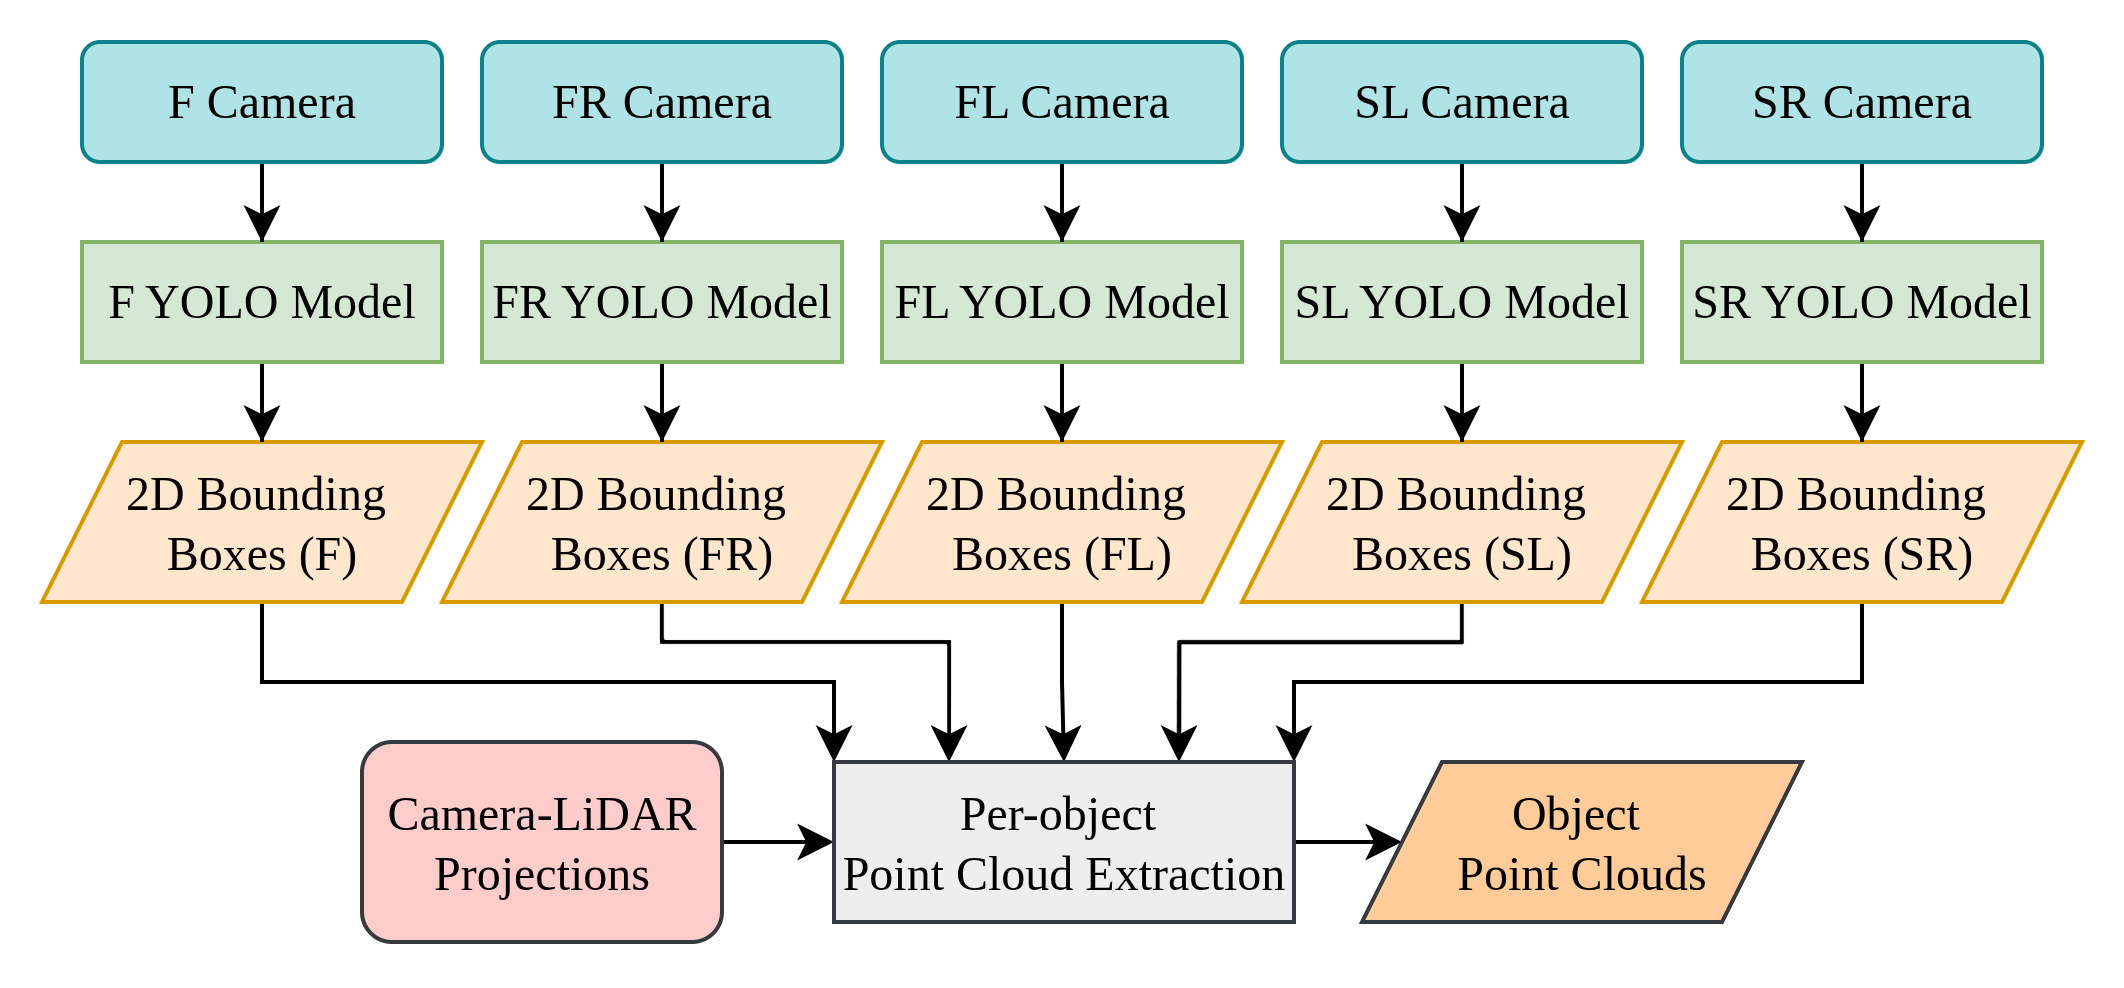
\includegraphics[scale=0.2]{gambar/object_pc.png}
  \caption{Process flow, gathering point clouds for each object}
  \label{fig:object_pc}
\end{figure}

Camera-LiDAR projections available with WOPD will be utilized to convert 2D bounding-box images into 3D Point Clouds for each object, as visualized by Figure~\ref{fig:object_pc}. This process is to be done by matching every pixel corresponding to the 2D object (every pixel inside the bounding box of a certain object in the image) into its corresponding LiDAR points. Then, to eliminate any background or foreground objects overlapping with the bounding box from the point cloud, the points' distance from the LiDAR is taken into account and those that fall outside percentiles \verb|min_p| and \verb|max_p| are discarded. Values for \verb|min_p| and \verb|max_p| are to be determined from a lightweight Artificial Neural Network (ANN), taking account the 2D inference class to produce a clean lidar point cloud for each object. 

\subsection{Modeling: 3D Bounding Box Generation}

\begin{figure}[H]
  \centering
  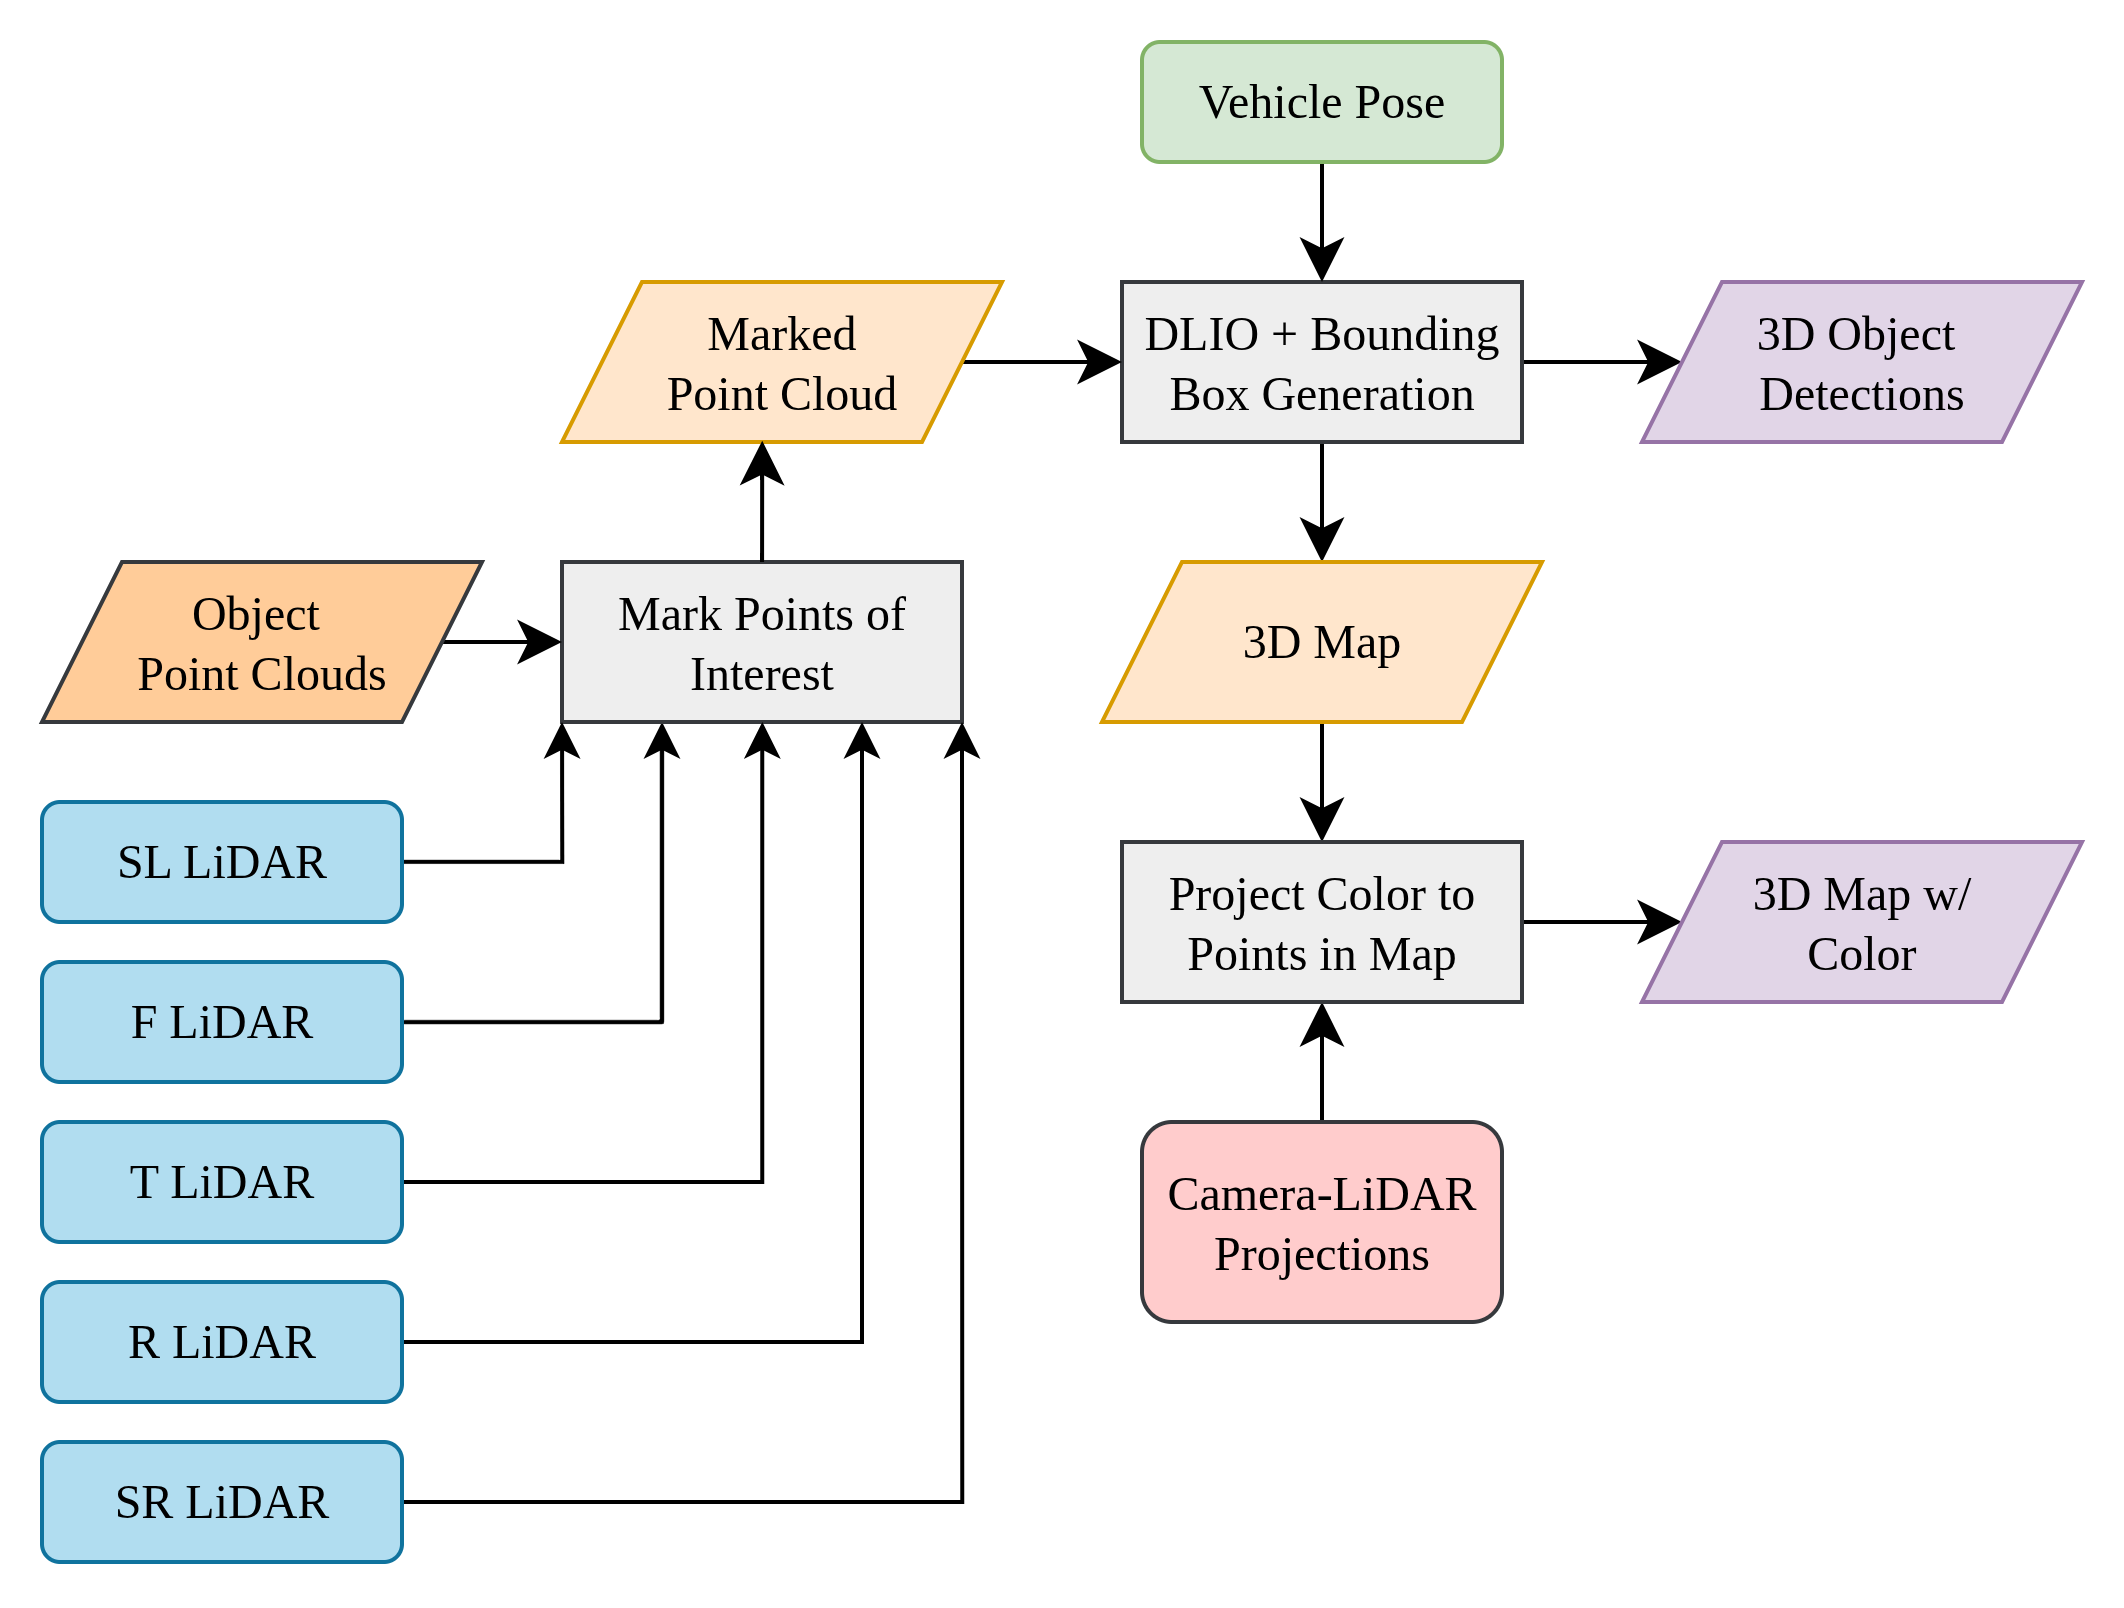
\includegraphics[scale=0.2]{gambar/detection_and_mapping.png}
  \caption{Modeling: 3D Object Detection and Mapping}
  \label{fig:detection_and_mapping}
\end{figure}

A combination between the lidar point cloud itself and vehicle pose data will be combined in order to create a high-precision 3D Map. The LiDAR point cloud data will be segmented using concave-hull and convex-hull K-Nearest Methods to extract reference objects (\emph{objects of interest}) from the environment. Changes in the orientation and position of each reference object will be used to estimate location changes. The IMU in this system serves to add context to the \emph{pose} transition between two instances of point cloud detection, improving the accuracy of orientation and position estimation for each object of interest. Figure~\ref{fig:detection_and_mapping} shows the process flow.

\section{Hardware Environment}

\subsection{NVIDIA AD103-400} 

\begin{figure}[H]
  \centering
  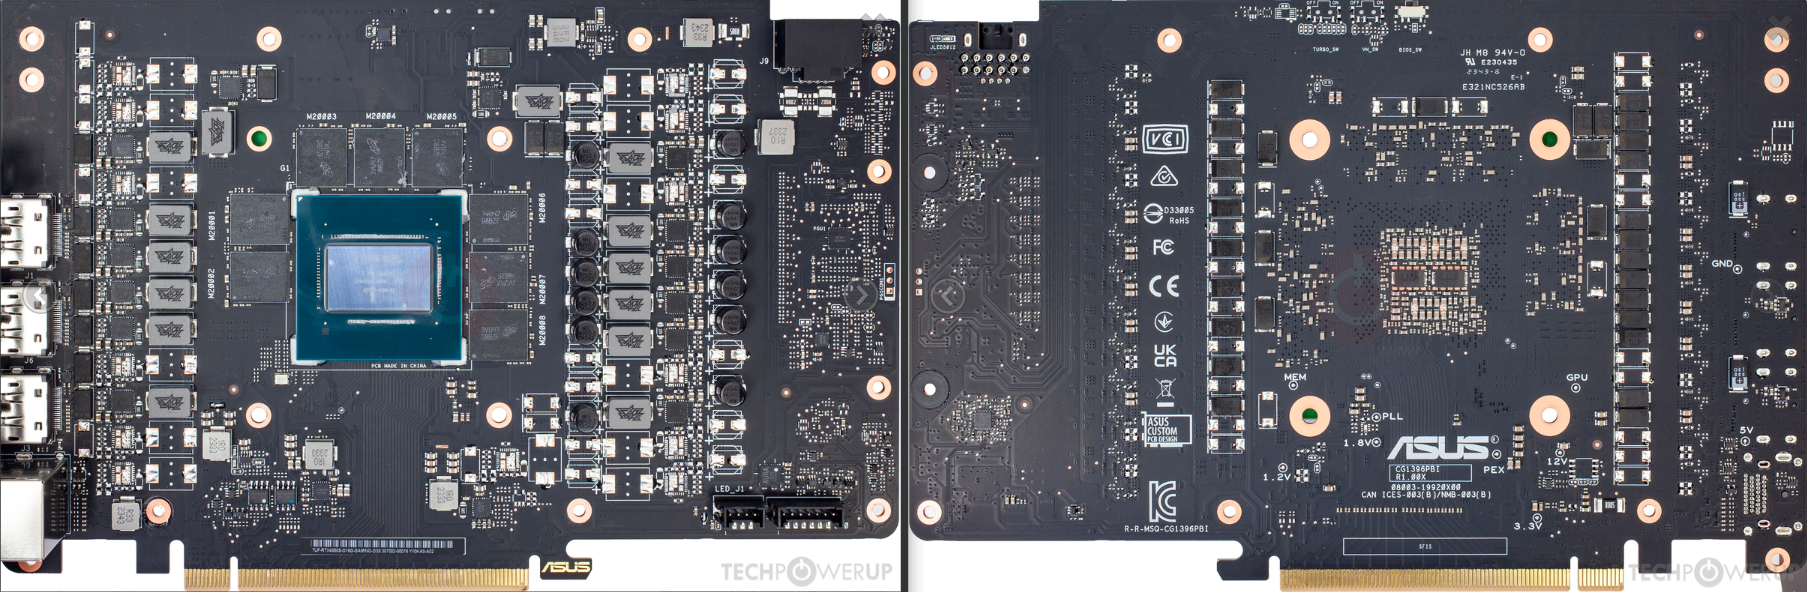
\includegraphics[scale=0.23]{gambar/ad103_400.png}
  \caption{Front view (left) and back view (right) of the NVIDIA AD103-400 GPU with ASUS-manufactured PCB}
  \label{fig:ad103_400}
\end{figure}

The NVIDIA AD103-400, commonly known as the RTX 4080 Super, is a consumer-grade GPU from NVIDIA. Due to its relative ease-of-access and significant computational capacity. The AD103-400 on an ASUS-manufactured motherboard (shown in Figure~\ref{fig:ad103_400}) will be used for training the multiple YOLO models as well as the lightweight ANN models used in RT-LIVO2DM. Table~\ref{tab:ad103_specifications} describes the specification of the AS103-400 in detail.

\begin{table}[h!]
\centering
\caption{Specifications of the NVIDIA AD103-400}
\label{tab:ad103_specifications}
\begin{tabular}{lcc}
\toprule
\textbf{Attribute} & \textbf{Value} \\
\midrule
GPU Model & NVIDIA AD103-400 \\
GPU Architecture & Ada Lovelace \\
CUDA Cores & 10,240 \\
Tensor Cores & 320 \\
Base Clock & 2.295 GHz \\
Boost Clock & 2.505 GHz \\
VRAM Capacity & 16 GB GDDR6X \\
Memory Interface Width & 256-bit \\
Memory Bandwidth & 736 GB/s \\
L2 Cache & 64 MB \\
TDP (Thermal Design Power) & 320 W \\
Compute Performance (FP32) & 52.22 TFLOPS \\
Manufacturing Process & TSMC 4N (4 nm) \\
\bottomrule
\end{tabular}
\end{table}

\subsection{NVIDIA Jetson AGX ORIN} 

\begin{figure}[H]
  \centering
  \includegraphics[scale=0.1]{gambar/jetson_agx_orin.png}
  \caption{NVIDIA Jetson AGX ORIN: with casing (left) and without casing (right)}
  \label{fig:jetson_agx_orin}
\end{figure}

NVIDIA Jetson AGX ORIN (as shown in Figure~\ref{fig:jetson_agx_orin}) is one of the variants in the NVIDIA Jetson family. This research will use Jetson AGX ORIN as the testing platform due to its comparable computational scale with the NVIDIA DRIVE ORIN, which is widely used in modern autonomous vehicle applications. Table~\ref{tab:jetson_agx_orin_specifications} details the technical specifications of the NVIDIA Jetson AGX ORIN. The Jetson AGX ORIN is pre-built with capabilities for hardware-wise down-throttling of computational capacity, making it a preferrable choice for inference hardware for this research, by consistently emulating different computational capacity scenarios.

\begin{table}[h!]
  \centering
  \caption{Specifications of the NVIDIA Jetson AGX Orin}
  \label{tab:jetson_agx_orin_specifications}
  \begin{tabular}{lcc}
  \toprule
  \textbf{Specification} & \textbf{Value} \\
  \midrule
  Processor & 12-core ARM Cortex-A78AE v8.2 64-bit CPU \\
  CUDA Cores & 2,048 \\
  Tensor Cores & 64 \\
  Memory & 64 GB LPDDR5  \\
  Storage & 64 GB eMMC 5.1 \\
  Memory Bandwidth & 204.8 GB/s \\
  AI Performance (INT8) & Up to 275 TOPS \\
  AI Performance (FP16) & Up to 137 TFLOPS \\
  Power Consumption & 15 W – 60 W (configurable) \\
  Networking & 10/100/1000 BASE-T Ethernet \\
  Form Factor & 100 mm × 87 mm \\
  Operating System & Ubuntu-based JetPack SDK \\
  \bottomrule
  \end{tabular}
\end{table}

\section{Implementation Approach}

\subsection{Data Extraction}
Algorithm~\ref{prog:waymo_get} outlines the process of developing a minimal reproducible workflow for downloading a \emph{training} or \emph{validation} shard.

\begin{algorithm}[H]
\caption{Minimal Workflow to Acquire and Inspect a Waymo Open Perception Shard}
  \label{prog:waymo_get}
  \begin{algorithmic}[1]
  \Require Internet connection, \texttt{gsutil}, Python~$\geq$3.8, TensorFlow~$\geq$2.11
  \Ensure Local directory \texttt{./wopd/training/} containing n shards and a verified frame count

  \State \textbf{Environment}:
  \State \quad \texttt{pip install waymo-open-dataset-tf-2-11-0} \Comment{or latest tag}

  \State \textbf{Select shards}:
  \State \quad $S \gets$ list of any n files matching 

  \texttt{gs://.../individual\_files/training/segment-*.tfrecord}

  \State \textbf{Download}:
  \State \quad \texttt{gsutil -m cp} $S$ \texttt{./wopd/training/}

  \State \textbf{Sanity check}:
  \State \quad $L \gets$ \texttt{glob("./wopd/training/segment-*.tfrecord")}
  \State \quad $D \gets$ \texttt{tf.data.TFRecordDataset}$(L)$
  \State \quad \textbf{print} ``Num. frames:'' $\sum_{\_ \in D} 1$
  \end{algorithmic}
\end{algorithm}

\subsection{Image Data Extraction}

Algorithm~\ref{prog:offline_extract} describes the outline of converting the collected shard/s into a directory of JPEG files and a manifest JSON file to be used for training purposes. The exact directory structure will follow the standard YOLO format for training.

\begin{algorithm}[H]
  \caption{Offline Pre-extraction (Training Mode)}
  \label{prog:offline_extract}
  \begin{algorithmic}[1]
  \Require List of shards $\mathcal{S}$, target camera $c$ (e.g. \texttt{FRONT})
  \Ensure Directory \texttt{./images/} of JPEG files and \texttt{manifest.json}

  \State $\mathcal{M} \gets [\;]$ \Comment{Empty JSON manifest}
  \For{shard $f \in \mathcal{S}$}
      \For{$(\text{img}, K, \text{labels})$ from \Call{FrameParser}{$f, c$}}
          \State $\text{frame\_id} \gets$ unique identifier from $f$
          \State write\_jpeg(img, \texttt{"./images/\{frame\_id\}.jpg"})
          \State $\mathcal{M}.\text{append}\bigl(\{\text{"file": } \ldots,\ \text{"labels": } \ldots\}\bigr)$
      \EndFor
  \EndFor
  \State flush\_json($\mathcal{M}$, \texttt{"manifest.json"})
  \end{algorithmic}
\end{algorithm}

% \begin{algorithm}[H]
% \caption{Online Streaming (Validation / Live Demo)}
% \label{prog:online_stream}
% \begin{algorithmic}[1]
% \Require List of shards $\mathcal{S}$, target camera $c$
% \Ensure Infinite generator of pre-processed RGB tensors

% \Function{waymo\_stream}{$\mathcal{S}, c$}
%     \For{shard $f \in \mathcal{S}$}
%         \For{$(\text{img}, \_, \_)$ from \Call{FrameParser}{$f, c$}}
%             \State $\text{tensor} \gets$ \Call{preprocess\_for\_yolo}{img} \Comment{resize, normalize, etc.}
%             \State \textbf{yield} tensor
%         \EndFor
%     \EndFor
% \EndFunction
% \end{algorithmic}
% \end{algorithm}

\subsection{Modeling: 2D Object Detection}

Algorithm~\ref{prog:yolo_loop} outlines the process of running a minimal YOLO inference loop on a running Waymo shard. The function \Call{waymo\_stream}{$\mathcal{S}, c$} is a generator that returns pre-processed RGB tensors from a shard. 

\begin{algorithm}[H]
\caption{Minimal YOLO Inference Loop}
\label{prog:yolo_loop}
\begin{algorithmic}[1]
\Require Trained YOLO model $\mathcal{M}$, generator \Call{waymo\_stream}{$\mathcal{S}, c$}
\Ensure Per-frame predictions $\mathcal{R}_t$

\State load $\mathcal{M} \gets$ \texttt{"yolov11n.pt"}
\For{tensor $T_t$ from \Call{waymo\_stream}{$\mathcal{S}, \text{"FRONT"}$}}
    \State $\mathcal{R}_t \gets$ \Call{predict}{$\mathcal{M}, T_t, \text{device="cuda:0"}$}
    \State \Call{post\_process}{$\mathcal{R}_t$} \Comment{project to 3D, log, etc.}
\EndFor
\end{algorithmic}
\end{algorithm}

\subsection{Modeling: Per-Object Point Cloud Extraction}

Algorithm~\ref{alg:pepce} describes the process flow of extracting per-object point cloud as a step in RT-LIVO2DM inference in detail.

\begin{algorithm}[H]
\caption{Per-object Point Cloud Extraction}
\label{alg:pepce}
\begin{algorithmic}[1]
\Require Set of 2D bounding boxes $\mathcal{B}$ (F, FR, FL, SL, and SR 2D Bounding Boxes) \\
         Lidar-camera projection function $P: (u, v, c) \rightarrow \mathbb{R}^3$ \\
         Pretrained ANN model $M$ for min/max percentile prediction
\Ensure Set $\mathcal{P}$ of refined 3D point clouds (one point cloud per bounding box)

\State $\mathcal{P} \gets \{\}$ \Comment{Initialize result set of point clouds}

\ForAll{bounding box $b_i \in \mathcal{B}$}
    \State $C_i \gets$ camera index where $b_i$ is detected
    \State $P_i \gets \{\}$ \Comment{Initialize point set for this box}
    \ForAll{pixels $(u, v)$ within $b_i$}
        \State $p \gets P(u, v, C_i)$ \Comment{Project pixel to 3D}
        \If{$p$ is valid}
            \State $P_i \gets P_i \cup \{p\}$
        \EndIf
    \EndFor

    \State $c_i \gets$ class label of detection $b_i$
    \State $d_i \gets$ distances of all points in $P_i$ to ego-vehicle

    \Comment{Use ANN model to determine percentiles based on class}
    \State $(\text{min}_p, \text{max}_p) \gets M(P_i, c_i)$
    \Comment{$M$ takes class label as input, returns two percentiles}

    \State $d_{\text{min}} \gets \text{percentile}(d_i, \text{min}_p)$
    \State $d_{\text{max}} \gets \text{percentile}(d_i, \text{max}_p)$

    \State $P_i \gets \{p \in P_i \mid d_{\text{min}} \leq \|p\| \leq d_{\text{max}}\}$
    \State $\mathcal{P} \gets \mathcal{P} \cup \{P_i\}$ \Comment{Append result}
\EndFor

\State \textbf{Output:} $\mathcal{P}$, a set of refined 3D point clouds per detected object
\end{algorithmic}
\end{algorithm}

\subsection{Modeling: 3D Bounding Box Generation}

Point cloud data from WOPD LiDAR sensors will be marked with an object label to determine which object (if any) each point belongs to. A modification of DLIO will be implemented to convert the marked point cloud into both 3D Bounding Boxes for each object and a 3D Map. The point cloud of each object will undergo a function involving Convex Hull + Minimum Volume Bounding Box to determine its corresponding 3D bounding box. This approach is similar to how one of the subsystems in DLIO (mentioned later) works, which allows for the segmentation of 3D objects from point cloud data without the need for significant computational resource. Algorithm~\ref{alg:3dbbox} describes the process in detail.

\begin{algorithm}[H]
  \caption{3D Bounding Box Generation}
  \label{alg:3dbbox}
  \begin{algorithmic}[1]
  \Require Point cloud $\mathcal{P}$ as a list of 3D points
  \Ensure Center $C$, Size $S$, Rotation matrix $R$
  \State Initialize empty point cloud object: $\mathcal{P}_{cd} \gets \texttt{PointCloud()}$
  \State Assign point data: $\mathcal{P}_{cd}.\texttt{points} \gets \texttt{Vector3dVector}(\mathcal{P})$
  \State Compute oriented bounding box: $\mathcal{B} \gets \mathcal{P}_{cd}.\texttt{get\_oriented\_bounding\_box}()$
  \State Extract center: $C \gets \mathcal{B}.\texttt{center}$
  \State Extract extent: $S \gets \mathcal{B}.\texttt{extent}$
  \State Extract rotation: $R \gets \mathcal{B}.\texttt{R}$
  \State \Return $C, S, R$
  \end{algorithmic}
\end{algorithm}